\documentclass{article}
\usepackage{amsmath}
\usepackage{amssymb}
\usepackage{tikz}
\usepackage{hyperref}
\hypersetup{
  colorlinks=true,
  linkcolor=blue
}

\renewcommand{\labelitemi}{-}
\renewcommand{\labelitemii}{+}

\title{Block Ciphers and DES}
\author{}
\date{2021-03-23}

\begin{document}
  \maketitle 
  \tableofcontents
  \break

  \section{Block ciphers}

  Block ciphers are symmetric ciphers which operate on groups of bits
  called \emph{blocks}.
  We could think of a block like an \emph{array} of bits.
  
  This means that both the encryption algorithm and the decryption
  algorithm take as input a block:

  \begin{center}
	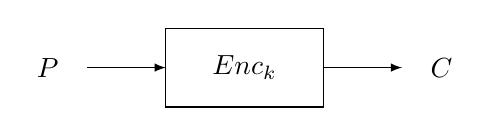
\begin{tikzpicture}
	  \draw[->,>=latex](-1, 0) -- (0, 0);	  
	  \draw[->,>=latex](2, 0) -- (3, 0);
	  \draw(-0, -.5) rectangle (2, .5);
	  \draw(1, 0) node {$Enc_{k}$};
	  \draw(-1.5, 0) node {$P$};
	  \draw(3.5, 0) node {$C$};
	\end{tikzpicture}
  \end{center}

  \begin{center}
	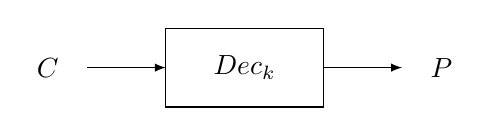
\begin{tikzpicture}
	  \draw[->,>=latex](-1, 0) -- (0, 0);	  
	  \draw[->,>=latex](2, 0) -- (3, 0);
	  \draw(-0, -.5) rectangle (2, .5);
	  \draw(1, 0) node {$Dec_{k}$};
	  \draw(-1.5, 0) node {$C$};
	  \draw(3.5, 0) node {$P$};
	\end{tikzpicture}
  \end{center}

  Where:
  $$
	P = 
	\begin{bmatrix}
	  x_{0} \\
	  x_{1} \\
	  \dots \\
	  x_{n}
	\end{bmatrix}
	\qquad
	C = 
	\begin{bmatrix}
	  y_{0} \\
	  y_{1} \\
	  \dots \\
	  y_{n}
	\end{bmatrix}
  $$

  Notice that the plaintext block and ciphertext block have the same
  length.

  \subsection{Rounds}

  A block algorithm is based on the repetition of short sequences of
  operations called \emph{rounds}.
  A round is a basic transformation which operates on a block. For
  example, an encryption algorithm could consist of three rounds: $C =
  R_{3} (R_{2}(R_{1}(P)))$. Each round should also have an
  \emph{inverse} in order to compute back the plaintext from the
  ciphertext: $P = R_{1}^{-1} (R_{2}^{-1}(R_{3}^{-1}(C)))$.
  
  There are two main techniques to build rounds:
  \emph{substitution-permutation networks} and \emph{Feistel
  schemes}.


  \subsubsection{Round keys and key schedule algorithm}

  Usually round functions ($R_{1},\dots R_{n}$) are the same, but they
  are parametrized by a \emph{round key}.
  A round key is a key which derives from the main key $K$.
  The same round function with different round keys will behave
  differently, and therefore will produce a different output blocks.

  An algorithm called \emph{key schedule} produces the round keys
  starting from the main key $K$.
  Round keys should always be different from each other in every round.
  

  \subsubsection{Substitution-permutation networks}  

  Substitution-permutation networks put together two important
  properties of cryptography\footnote{The terms \emph{confusion} and
  \emph{diffusion} were introduced by Claude Shannon.}:

  \begin{description}
	\item[Confusion:] the input (plaintext and key) undergoes
	  complex transformations, which make the relationship between the
	  statistics of the ciphertext and the value of the encryption key
	  as complex as possible. 
	\item[Diffusion:] the transformations depend equally on all bits
	  of the input, i.e. the ciphertext doesn't reflect the
	  statistical properties of the plaintext.
  \end{description}

  In a block cipher, a simple diffusion element is the bit
  \emph{permutation} (which is used frequently in DES),
  while confusion is achieved
  by the use of \emph{substitution} (used both in DES and in AES).

  \paragraph{Substitution:}
  
  Substitution boxes (S-boxes) 
  are small lookup tables that transform chunks of
  4 or 8 bits. For example, the 4-bit nibble $0000$ could be mapped to
  $0011$, while $0101$ could be mapped to $0110$, and so on.
  These S-boxes must be cryptographically strong (i.e. they
  should be as nonlinear as possible and have no statistical bias).

  \paragraph{Permutation:}
  The permutation could simply constist of a permutation of the bits,
  which is easy to implement but doesn't create to much diffusion.
  In practice different ciphers use operations from the linear algebra 
  to mix up the bits, like matrix-multiplications, and so on.
  Those operations create strong dependencies with all the bits of the
  input, and therefore ensure strong diffusion.

  \subsubsection{Feistel schemes}

  A Feistel scheme works as follows.:  
  \begin{enumerate}
	\item The input block is splitted in two halves, $L$ and $R$
	\item $L$ is XOR-ed with $F(R)$, where $F$ is a
	  substitution-permutation round
	\item $L$ and $R$ are swapped
	\item Step 2. and 3. are repeated a bunch of times
	\item $L$ and $R$ are merged into the output block
  \end{enumerate}

  \begin{center}
	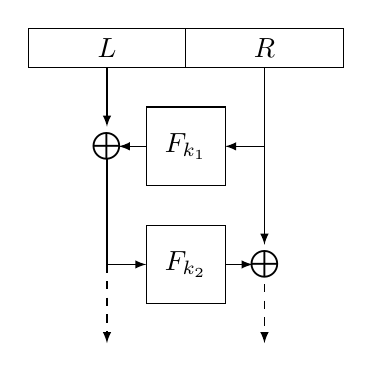
\begin{tikzpicture}
	  \draw(0, 3) rectangle (2, 3.5); 	  
	  \draw(1, 3.25) node {$L$};
	  \draw(2, 3) rectangle (4, 3.5);
	  \draw(3, 3.25) node {$R$};
	  \draw[->,>=latex](1, 3) -- (1, 2.25); %left arrow
	  \draw(1, 2) node {$\bigoplus$};
	  % arrow from R to F
	  \draw[->,>=latex](3, 3) -- (3, 2) -- (2.5, 2);
	  % F block
	  \draw(1.5, 1.5) rectangle (2.5, 2.5);
	  \draw(2, 2) node {$F_{k_{1}}$};
	  % arrow from F to XOR
	  \draw[->,>=latex](1.5, 2) -- (1.15, 2);
	  % arrow from XOR to F2
	  \draw(1.5, 0) rectangle (2.5, 1);
	  % XOR 2
	  \draw(3, .5) node {$\bigoplus$};
	  \draw[->,>=latex](3, 2) -- (3, .75);
	  \draw[->,>=latex](1, 1.85) -- (1, .5) -- (1.5, .5);
	  \draw(2, .5) node {$F_{k_{2}}$};
	  \draw[->,>=latex](2.5, .5) -- (2.85, .5);
	  \draw[->,>=latex,dashed](1, .5) -- (1, -.5);
	  \draw[->,>=latex,dashed](3, .25) -- (3, -.5);
	\end{tikzpicture}
  \end{center}

  Notice that $F_{k_{1}}$ and $F_{k_{2}}$ are actually the same
  function, they just take as input different round keys $K_{1}$ and
  $K_{2}$, which come from the key scheduling algorithm.
  

  \subsection{4$\times$4 S-box cipher}

  Howard M. Heys introduced this simple substitution-permutation based block 
  cipher in his lectures \emph{A Tutorial on Linear and Differential Algebra}.

  \paragraph{Substitution}
  \begin{itemize}
	\item The algorithm operates on 16-bit blocks.
	\item Each block is broken into four 4-bit sub-blocks.
	\item Each sub-block is fed into a $4\times4$ S-box (a
	  substitution-box with 4 input bits and 4 output bits). 
	\item In this case we use the same mapping for all
	  S-boxes\footnote{In DES all the S-boxes in a round are
	  different.}
	\item The S-box performs a \emph{nonlinear} mapping, i.e. the
	  output bits cannot be represented as a linear function of the
	  input bits.
  \end{itemize}

  The S-box used is the following:
  \begin{center}
	\begin{tabular}{|c|c|c|c|c|c|c|c|c|c|c|c|c|c|c|c|c|}
	  \hline
	  input & 0 & 1 & 2 & 3 & 4 & 5 & 6 & 7 & 8 & 9 & A & B & C & D & E & F \\
	  \hline
	  output & E & 4 & D & 1 & 2 & F & B & 8 & 3 & A & 6 & C & 5 & 9 &
	  0 & 7 \\
	  \hline
	\end{tabular}
  \end{center}

  You can verify that the mapping is nonlinear\footnote{A linear
  function maps a certain value $x$ into $k x$, where
  $k \in \mathbb{R}^{n}$} by simply observing
  that the number 0 is mapped to the hexadecimal value E 
  (which is 14 in decimal), while a linear function always maps the
  null-element 0 into 0 itself.
  Also, the mapping is not \emph{affine}:\footnote{An affine function
  maps a certain element $x$ into $kx+c$ where $k, c \in
  \mathbb{R}^{n}$.} while $\textrm{E}_{hex}$ = $14_{dec}$ = 0 + 14,
  instead $4 \neq 1 + 14$.

  \paragraph{Permutation}
  
  The permutation consists of a simple transposition of the bits, or
  the permutation of the bit positions.
  In the following \emph{permutation table} we represent for each
  input bit the position that it will take in the output (for example,
  the bit 2 is moved to position 5). 
  We stick with the author convention, in which $1$ is the
  rightmost bit and $16$ is the leftmost bit.
  \begin{center}
	\begin{tabular}{|c|c|c|c|c|c|c|c|c|c|c|c|c|c|c|c|c|}
	  \hline
	  input & 1 & 2 & 3 & 4 & 5 & 6 & 7 & 8 & 9 & 10 & 11 & 12 & 13 & 14 & 15& 16 \\
	  \hline
	  output & 1 & 5 & 9 & 13 & 2 & 6 & 10 & 14 & 3 & 7 & 11 & 15 & 4 & 8 &
	  12 & 16 \\
	  \hline
	\end{tabular}
  \end{center}
  
  \paragraph{Key mixing}

  To achieve key mixing, data blocks are XOR-ed with a round key
  before being fed into a S-box.


  % There are two main techniques to build a round:
  % \emph{substitution-permutation networks} and \emph{Feistel schemes}.
  
  \section{DES}
  
  \subsection{History} 

  In 1972 the US National Bureau of Standards (NBS, currently NIST)
  initiated a request for proposal for a standardized cipher in the
  USA. Up to this point in time cryptography had always been kept
  secret. By the early 70s, however, cryptography had become of
  crucial importance for a variety of commercial applications such as
  banking.

  The winning proposal selected in 1974 came from a team of
  cryptographers working at IBM.
  They submitted an algorithm based on the family of Feistel's ciphers 
  called \emph{Lucifer}, developed in the late 60s.

  In 1977 the NBS finally released all specifications of the IBM cipher 
  (which meanwhile had passed through some modifications) as 
  \emph{Data Encryption Standard} to the public. 
  However, the motivation for parts of the DES design\footnote{i.e.
  the design criteria.} were never officially released.
  During the following years, with the increase of personal computers
  in the early 80s, it became easier to analyze the inner structure of
  the cipher. However, no serious weaknesses were found until 1990.

  In 1999 DES was replaced by AES.

  \subsection{Description}

  DES is a symmetric block cipher which encrypts 64-bit blocks with a
  56-bit key. 

  \begin{center}
	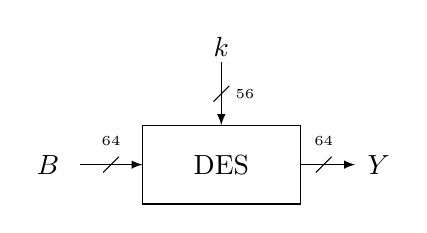
\begin{tikzpicture}
	  \draw(0, 0) rectangle (2,1);
	  \draw(1, 2) node {$k$};
	  \draw[->,>=latex](1, 1.8) -- (1, 1);
	  \draw(.9, 1.3) -- (1.1, 1.5);
	  \draw(1.3, 1.4) node {\tiny{56}};
	  \draw(1, .5) node {DES};
	  \draw[->,>=latex](-.8, .5) -- (0, .5);
	  \draw(-.5, .4) -- (-.3, .6);
	  \draw(-1.2, .5) node {$B$};
	  \draw(-.4, .8) node {\tiny{64}};
	  \draw[->,>=latex](2, .5) -- (2.7, .5);
	  \draw(2.2, .4) -- (2.4, .6);
	  \draw(2.3, .8) node {\tiny{64}};
	  \draw(3, .5) node {$Y$};
	\end{tikzpicture}
  \end{center}


  Each block passes through an initial bitwise permutation $IP$, then 
  16 rounds which all perform the identical operation, and eventually 
  a final bitwise permutation $IP^{-1}$, which is the inverse of the
  initial permutation $IP$.
  
  \begin{center}
	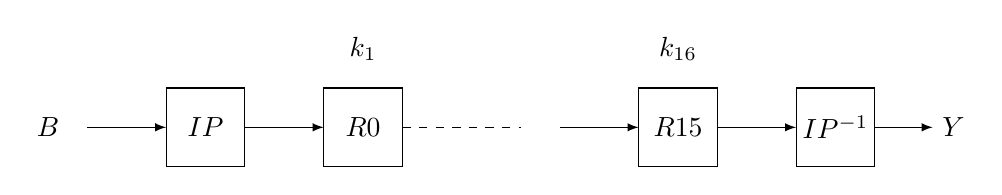
\begin{tikzpicture}
	  \draw(-1.5, .5) node(x) {$B$};  
	  \foreach \i / \txt in {0/$IP$,1/$R0$,3/$R15$,4/$IP^{-1}$}
	  {
		\draw(\i*2, 0) rectangle (\i*2+1, 1);
		\draw[->,>=latex](2*\i-1, .5) -- (2*\i, .5);
		\draw(\i*2+.5, .5) node {\txt};
	  }
	  \draw(2.5, 1.5) node {$k_{1}$};
	  \draw(6.5, 1.5) node {$k_{16}$};
	  \draw[dashed](3, .5) -- (4.5, .5);
	  \draw(10, .5) node(y) {$Y$};
	  \draw[->,>=latex](9, .5) -- (y);
	\end{tikzpicture}
  \end{center}

  In each round a different round key $k_{i}$ derived from the main
  key $k$ (with a key schedule) is used.
  Each DES round implements a Feistel scheme.
  
  \subsubsection{Internal permutation}

  The internal permutation $IP$ maps each input bit to an output bit.
  This doesn't increase security, it's just to arrange the plaintext. 
  The final permutation $IP^{-1}$ performs the reverse mapping.
  The following tables show the final position of each bit from $0$ to 63.
  The \hyperlink{appendix}{appendix} shows both the $IP$ and the
  $IP^{-1}$ structure.

  \subsubsection{The $f$ function}

  The Feistel function $f$ plays a crucial role for the security 
  of the DES cipher. In round $i$ it takes the right half 
  $R_{i-1}$ (32-bits) of the 
  output of the previous step and the round key $k_{i}$.
  The output is then XOR-ed with the left half of the previous step
  $L_{i-1}$ (32-bits).
  
  \begin{itemize}
	\item First, the 32-bit input is expanded to 48-bits by
	  partitioning the input into eight 4-bit blocks which are
	  expandend to 6-bit blocks with a $E$-box (a special type of
	  permutation). You can find the $E$-box in the
	  \hyperlink{appendix}{appendix}.

  
  \item Then the 48-bit result of the expansion is XOR-ed with the
	round key $k_{i}$, and the eight 6-bit blocks are fed into eight
	different S-boxes; each S-box maps a 6-bit block to a 4-bit
	block\footnote{Eight 4$\times$6 tables were close to the
	maximum size which could be fit on a single integrated circuit in
	1974.}.
	Each S-box contains $2^{6} = 64$ entries. Each entry is a 4-bit
	  value. The \hyperlink{appendix}{appendix} shows all the S-boxes.

	  The \emph{design criteria} behind the S-boxes are the following:
	  \begin{enumerate}
		\item Each S-box has 6 input bits and 4 output bits.
		\item No output bit of an S-box should be too close to a linear
		  combination of the input bits.
		\item If the lowest and highest bits of the input are fixed
		  and the four middle bits are varied, each of the possible
		  4-bit output values must occur exactly once.
		\item If two input to an S-box differ in exactly one bit,
		  their outputs must differ in at least two bits.
		\item If two inputs to an S-box differ in the two middle bits,
		  their outputs must differ in at least two bits.
		\item If two inputs to an S-box differ in their first two bits
		  and are identical in their last two bits, the two outputs
		  must be different.
		\item For any nonzero 6-bit difference between inputs, no more
		  than 8 of the 32 pairs of inputs exhibiting that difference
		  may result in the same output difference.
		\item A collision (zero output difference) at the 32-bit
		  output of the eight S-boxes is only possible for three
		  adjacent S-boxes.
	  \end{enumerate}

	  See \hyperlink{ex427}{Exercise 4.2.7} in which properties 3, 4,
	  5, 6 are checked.

	\item Finally, the 32-bit output passes through the $P$
	  permutation (see the \hyperlink{appendix}{appendix}).
	  This permutation introduces diffusion, because the four output
	  bits of each S-box are permuted in such a way that they affect
	  several different S-boxes in the following round.

	  The diffusion created by expansion, S-boxes and the $P$
	  permutation guarantees that each bit at the end of the fifth
	  round is a function of every plaintext bit and every key bit
	  (\emph{avalanche effect}).

  \end{itemize}

  The following picture represents the internal structure of the $f$
  function:

  \begin{center}
	\begin{tikzpicture}
	  \draw(-1.25, .25) node(r) {$R_{j}$};
	  \draw(0, 0) rectangle (1, .5) node[pos=.5] {$E$};
	  \draw[->,>=latex](-1, .25) -- (0, .25) node[midway, above]
	  {\tiny{32}} node[midway] {\tiny{/}};
	  \draw[->,>=latex](1, .25) -- (2, .25) node[midway,above]
	  {\tiny{48}} node[midway]{\tiny{/}};
	  \draw(2.2, .25) node {$\bigoplus$};
	  \draw(2.4, .25) -- (3, .25);
	  \draw[->,>=latex](2.2, 1) -- (2.2, .5);
	  \draw(2.2, 1.25) node(name) {$k_{j+1}$};
	  \draw(3, 3.75) -- (3, -3.25);
	  \foreach \i in {1,...,8}
	  {
		\draw[->,>=latex](3, 4.75-\i) -- +(1, 0) node[midway]
		{\tiny{/}} node[midway, above] {\tiny{6}};
		\draw(5, 4.75-\i) -- +(1, 0) node[midway] {\tiny{/}}
		node[midway,above] {\tiny{4}};
		\draw(4, 4.5-\i) rectangle +(1,.5) node[midway] {$S_{\i}$};
	  }
	  \draw(6, 3.75) -- (6, -3.25);
	  \draw[->,>=latex](6, .25) -- +(.5, 0);
	  \draw(6.5, 0) rectangle +(1, .5) node[midway] {$P$};
	  \draw[->,>=latex](7.5, .25) -- +(1, 0) node[midway]{\tiny{/}}
	  node[midway,above] {\tiny{32}};
	\end{tikzpicture}
  \end{center}

  See \hyperlink{ex4211}{Exercise 4.2.11} for an example of
  computation with the $f$ function.

  \subsubsection{The importance of being nonlinear}

  The S-boxes are at the core of DES in terms of cryptographic
  strength, because they produce confusion and are the \emph{only} 
  nonlinear element in the algorithm, i.e.:
  $$
	S(a) \oplus S(b) \neq S(a \oplus b)
  $$

  Why is nonlinearity so crucial? With a nonlinear building block, an
  attacker could express the DES input and output with a system of
  linear equations where the key bits are the unknowns. Such systems
  can easily be solved. S-boxes were carefully designed to
  prevent advanced mathematical attacks, such as \emph{differential
  cryptanalysis}.
  
  See \hyperlink{ex428}{Exercise 4.2.8} and \hyperlink{ex429}{Exercise
  4.2.9}.
  
  \subsection{Key schedule}

  The key schedule derives 16 round keys of from the main key $k$,
  each one consisting of 48-bits. 

  First, note that the DES input key is often stated as 64-bit, but
  every 7 bits there's an odd parity bit for the previous 7 bits.
  It's not clear why DES was specified that way, however the eight
  parity bits are not part of the actual key, they do not improve
  security, and therefore DES is a
  56-bit key cipher, not a 64-bit one.

  \begin{itemize}
	\item The parity bit are first removed from the key. Then the remaining
	  bits go through a permutation $PC-1$ (where $PC-1$ stands for
	  \emph{permuted choice one}). This permutation is shown in the
	  \hyperlink{appendix}{appendix}.
	\item The result is split into two halves $C_{0}$ and $D_{0}$.
	  The two 28-bit halves are cyclically shifted according to the
	  following rules:
	  \begin{itemize}
		\item In rounds $i = 1,2,9,16$ the two halves are rotated left
		  by one bit.
		\item In the other rounds, the two halves are rotated left by
		  two bits.
	  \end{itemize}
	\item To generate the 48-bit round keys $k_{i}$, the two halves
	  are permuted again with $PC-2$ (\emph{permuted choice 2}, see
	  \hyperlink{appendix}{appendix}), which
	  ignores the following bits: \texttt{9, 18, 22, 25, 35, 38, 43, 54}.
  \end{itemize}

  \subsection{Decryption}

  One advantage of DES is that decryption is the same function as
  encryption. This is because DES is based on a Feistel network.
  The only difference is the key schedule: the round keys are provided
  in reverse order (i.e. in round 1 round key 16 is needed, in round 2
  key 15, and so on).

  Because the total nubmber of rotations in the key schedule algorithm
  is 28, we have an interesting property: $C_{0} = C_{16}$ and $D_{0}
  = D_{16}$.
  Therefore, $k_{16}$ can be directly derived after
  $PC-1$\footnote{From now, we will omit the ‘-’ for clarity reasons.}:
  $$
	k_{16} = PC2(C_{16},D_{16}) = PC2(C_{0}, D_{0}) = PC2(PC1(k))	
  $$

  $k_{15}$ can be derived from $C_{16}, D_{16}$ through cyclic right
  shifts ($RS_{i}$):
  $$
	k_{15} = PC2(C_{15}, D_{15}) = PC2(RS_{2}(C_{16}),~
	RS_{2}(D_{16})) =
	PC2(RS_{2}(C_{0}), RS_{2}(D_{0}))
  $$

  \begin{itemize}
	\item In round 1 the key is not rotated.
	\item In rounds 2, 9 and 16 the two halves are rotated right by
	  one bit.
	\item In the other rounds the two halves are rotated right by two
	  bits.
  \end{itemize}
  
  \subsection{DES security}

  Ciphers can be attacked in several ways. With respect to
  cryptographic attacks, we distinguish between \emph{exhaustive key
  search} (or \emph{brute-force attacks}) and \emph{analytical
  attacks}.

  Although current analytical attacks against DES are not very
  efficient, DES can relatively easily be broken with an exhaustive
  key-search attack.
  This means that plain DES is not to be considered secure anymore.

  RSA security proposed several challenges to break DES, in order to
  prove that a 56-bit key is too short. During DES challenge III (1999),
  the EFF\footnote{Electronic Frontier Foundation.} decrypted a
  DES-encrypted message in 22 hours and 15 minutes by using Deep Crack, a 
  custom specifically built microchip.

  \subsubsection{3DES}

  A much stronger version of DES is 3DES, which consists of three
  subsequent DES encryptions with keys $k_{1}$, $k_{2}$, $k_{3}$.
  Usually 3DES is also implemented as EDE, i.e. the message is first
  encrypted with $k_{1}$, then decrypted with $k_{2}$ and finally
  encrypted with $k_{3}$.

  3DES seems resistant to both brute-force attacks and any known
  analytical attack.

  \subsubsection{2DES and meet-in-the-middle attack}
  
  We saw that 3DES is considered enough secure, but one could ask “Why
  not 2DES?”.
  The reason is quite simple: every block encryption algorithm, if
  applied two times, is vulnerable to the
  \emph{meet-in-the-middle-attack}.

  Let's consider a keylength of $\kappa$. Suppose that we first
  encrypt a plaintext by using a key $k_{1}$ and then we encrypt the
  ciphertext by using a key $k_{2}$.

  \begin{center}
	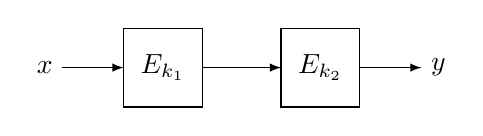
\begin{tikzpicture}
	  \draw(0, 0) node(x) {$x$};
	  \draw[->,>=latex](x) -- (1, 0);
	  \draw(1, -.5) rectangle (2, .5);
	  \draw(1.5, 0) node {$E_{k_{1}}$};
	  \draw[->,>=latex](2, 0) -- (3, 0);
	  \draw(3, -.5) rectangle (4, .5);
	  \draw(3.5, 0) node {$E_{k_{2}}$};
	  \draw(5, 0) node(y) {$y$};
	  \draw[->,>=latex](4, 0) -- (y);
	\end{tikzpicture}
  \end{center}

  A plain brute-force attack would require us to search through all
  possible combination of both keys, i.e. the effective key length
  would be $2\kappa$, and an exhaustive search would require
  $2^{\kappa} \cdot 2^{\kappa} = 2^{2\kappa}$ encryptions. 

  The meet-in-the-middle attack requires much more computational
  power:
  \begin{itemize}
	\item We (the adversary) know both the plaintext $x$ and the
	  ciphertext $y$.
	\item We first compute $2^{\kappa}$ encryptions of the
	  plaintext $x$, one  for each possible value of the key. 
	  We build a lookup table with all the encrypted values, indexed
	  by the value of $k_{1}$ that we used. 
	  In the case of DES, this would consist in $2^{56}$ operations.
	\item Then we start decrypting the ciphertext $y$ with all possible
	  values of the key $k_{2}$ ($2^{\kappa}$). 
	  If we find a match inside the lookup
	  table, then we have the key $k_{2}$. Not only: remember that the
	  lookup table is indexed by the value of $k_{1}$, this means that
	  we also have $k_{1}$. 
  \end{itemize}

  In the end, in the worst case we perform $2^{\kappa} + 2^{\kappa} =
  2\cdot 2^{\kappa} = 2^{\kappa + 1}$ operations, which are definitely
  less than $2^{2 \kappa}$.
  That's why double-encryption should be avoided with all the block
  ciphers.

  \paragraph{Example:}

  Let's say we have a plaintext $p$ and a ciphertext
  $c$.
  First we must encrypt $p$ with all possible $2^{\kappa}$ values of
  the key\footnote{For the sake of simplicity we consider just the
  decimal values.}:
  \begin{center}
	\begin{tabular}{|c|c|}
	  \hline
	  \texttt{k} & $\mathtt{Enc_{k}(p)}$ \\
	  \hline
	  \texttt{0} & \texttt{31269} \\
	  \hline
	  \texttt{1} & \texttt{161804} \\
	  \hline  
	  \dots & \dots \\
	  \hline
	  \dots & \dots \\
	  \hline
	  \texttt{$\mathtt{2^{\kappa-2}}$} & \texttt{21838121} \\
	  \hline
	  \texttt{$\mathtt{2^{\kappa-1}}$} & \texttt{193490} \\
	  \hline
	\end{tabular}
  \end{center}
  
  Then we start decrypting $c$ with all the possible $k_{2}$ key values.
  $$
	\mathtt{k=0} \Rightarrow \mathtt{Dec_{k}(c) = 1235443} 
  $$
  $$
	\mathtt{k=1} \Rightarrow \mathtt{Dec_{k}(c) = 21838121}
  $$

  We're lucky! It took us just two additional decryption to find a
  match. We look in the table and we see that the value
  \texttt{21838121} is in position $2^{\kappa-2}$. 
  In the end, the key $k_{1}$ is equal to $2^{\kappa-2}$, while the key $k_{2}$ is
  equal to 1, and we performed just $2^{\kappa} + 2$ computations.


  \section{Exercises}

  \hypertarget{ex427}{\paragraph{Exercise 4.2.7}}

  Check properties 3, 4, 5, 6 for S-box $S_{1}$.

  \begin{itemize}
	\item (3) It's easy to check that each row contains different
	  numbers. This means that for a fixed pair (first bit - last bit)
	  there are not two different middle bits configurations that produce the
	  same output.
	\item (4) Let's consider all the inputs which differ in exactly
	  one bit; you can check that the corresponding output bits will
	  differ in at least two bits. Let's take as an example the two
	  inputs 000000, which is mapped to 
	  $14 = 1110_{2}$, and 000001, which is mapped
	  to $0 = 0000_{2}$. While 000000 and
	  000001 differ in one bit, 1110 and
	  0000 differ in three bits.
	\item (5) Take as an example 000000, which is mapped to
	  $14 = 1110_{2}$ and 001100, which is mapped to 
	  $11 = 1011_{2}$. As you can see 1110 and
	  1011 differ in two bits.
	\item (6) Take as an example 000000, which is mapped to
	  $14 = 1110_{2}$ and 110000, which is mapped to
	$15 = 1111_{2}$. The output is clearly different.
  \end{itemize}

  \hypertarget{ex428}{\paragraph{Exercise 4.2.8}}

  Check that $S_{1}(4) \oplus S_{1}(23) \neq S_{1} (4 \oplus 23)$.

	  $$
		4 = 000100_{2}
		\qquad
		23 = 010111_{2}
	  $$
	  $$
		S_{1}(4) = 13 = 1101_{2}
		\qquad
		S_{1}(23) = 15 = 1111_{2}
	  $$
	  $$
		S_{1}(4 \oplus 23) = S_{1}(010011) = 6 = 0110_{2}
	  $$
	  $$
		S_{1}(4) \oplus S_{1}(23) = 0010_{2} = 2
	  $$
	  $$
		2 \neq 6
	  $$

	\hypertarget{ex429}{\paragraph{Exercise 4.2.9}}

	Check $S_{1}(0) \neq 0$. This shows that $S_{1}$ is non linear.
	$$
	  S_{1}(0) = 14 \neq 0
	$$

  \hypertarget{ex4211}{\paragraph{Exercise 4.2.11}}

  Compare the output of $f$ for inputs $R_{j} = 0$ and $R'_{j} = 1$
  with $k_{j+1} = 0$.

  \begin{itemize}
	\item First we compute the expansion through the $E$-box of both
	  $R_{j}$ and $R'_{j}$:
	  $$
		E(R_{j}) = 000\dots000 = 0^{48} 
		\qquad 
		E(R'_{j}) = 111\dots111 = 1^{48}
	  $$

	\item Then the expanded blocks are XOR-ed with the key $k_{j+1} =
	  0^{48}$:
	  $$
		E(R_{j})\oplus k_{j+1} = 0^{48}
		\qquad
		E(R'_{j})\oplus k_{j+1} = 1^{48}
	  $$

	\item Now we divide the 48-bit blocks in eight 6-bit sub blocks,
	  which are sent to the S-boxes. In this the sub blocks $B_{j}$ are all
	  the same:
	  $$
		B_{j} = 0^{6}
		\qquad
		B'_{j} = 1^{6}
	  $$
	  Let's apply the S-boxes to each block:
	  \begin{center}
		\begin{tabular}{crr}
		  $S_{1}(B_{j}) = $ & $14 = $ & $1110$ \\
		  $S_{2}(B_{j}) = $ & $15 = $ & $1111$ \\
		  $S_{3}(B_{j}) = $ & $10 = $ & $1010$ \\
		  $S_{4}(B_{j}) = $ & $7  = $ & $0111$ \\
		  $S_{5}(B_{j}) = $ & $2  = $ & $0010$ \\
		  $S_{6}(B_{j}) = $ & $12 = $ & $1100$ \\
		  $S_{7}(B_{j}) = $ & $4  = $ & $0100$ \\
		  $S_{8}(B_{j}) = $ & $13 = $ & $1101$ \\
		\end{tabular}
		\qquad
		\begin{tabular}{crr}
		  $S_{1}(B'_{j}) = $ & $13 = $ & $1101$ \\
		  $S_{2}(B'_{j}) = $ & $9  = $ & $0101$ \\
		  $S_{3}(B'_{j}) = $ & $12 = $ & $1100$ \\
		  $S_{4}(B'_{j}) = $ & $14 = $ & $1110$ \\
		  $S_{5}(B'_{j}) = $ & $3  = $ & $0011$ \\
		  $S_{6}(B'_{j}) = $ & $13 = $ & $1101$ \\
		  $S_{7}(B'_{j}) = $ & $12 = $ & $1100$ \\
		  $S_{8}(B'_{j}) = $ & $11 = $ & $1011$ \\
		\end{tabular}
	  \end{center}

	\item Finally, we apply $P$ to the concatenation of all the bits:
	  $$
		P(11101111101001110010110001001101) = 
	  $$
	  $$
		= f(R_{j}) =  11011000110110001101101110111100
	  $$
	  $$
		P(11010101110011100011110111001011) =
		$$
	  $$
		= f(R'_{j}) = 00111000110100111111100111011011
	  $$

  \end{itemize}



  \appendix
  \hypertarget{appendix}{\section{Appendix}}

  Read from left to right, top to bottom.

  \begin{center}
	$IP$ \\
	\vspace{10pt}
	\begin{tabular}{|cccccccc|}
	  \hline
	  \texttt{58} & \texttt{50} & \texttt{42} & \texttt{34} & \texttt{26} & \texttt{18} & \texttt{10} & \texttt{2} \\
	  \hline
	  \texttt{60} & \texttt{52} & \texttt{44} & \texttt{36} & \texttt{28} & \texttt{20} & \texttt{12} & \texttt{4} \\
	  \hline
	  \texttt{62} & \texttt{54} & \texttt{46} & \texttt{38} & \texttt{30} & \texttt{22} & \texttt{14} & \texttt{6} \\
	  \hline
	  \texttt{64} & \texttt{56} & \texttt{48} & \texttt{40} & \texttt{32} & \texttt{24} & \texttt{16} & \texttt{8} \\
	  \hline
	  \texttt{57} & \texttt{49} & \texttt{41} & \texttt{33} & \texttt{25} & \texttt{17} & \texttt{9} & \texttt{1} \\
	  \hline
	  \texttt{59} & \texttt{51} & \texttt{43} & \texttt{35} & \texttt{27} & \texttt{19} & \texttt{11} & \texttt{3} \\
	  \hline
	  \texttt{61} & \texttt{53} & \texttt{45} & \texttt{37} & \texttt{29} & \texttt{21} & \texttt{13} & \texttt{5} \\
	  \hline
	  \texttt{63} & \texttt{55} & \texttt{47} & \texttt{39} & \texttt{31} & \texttt{23} & \texttt{15} & \texttt{7} \\
	  \hline
	\end{tabular}
  \end{center}

  \begin{center}
	$IP^{-1}$ \\
	\vspace{10pt}
	\begin{tabular}{|cccccccc|}
	  \hline
\texttt{40} & \texttt{8} & \texttt{48} & \texttt{16} & \texttt{56} & \texttt{24} & \texttt{64} & \texttt{32} \\
	  \hline
\texttt{39} & \texttt{7} & \texttt{47} & \texttt{15} & \texttt{55} & \texttt{23} & \texttt{63} & \texttt{31} \\
	  \hline
\texttt{38} & \texttt{6} & \texttt{46} & \texttt{14} & \texttt{54} & \texttt{22} & \texttt{62} & \texttt{30} \\
	  \hline
\texttt{37} & \texttt{5} & \texttt{45} & \texttt{13} & \texttt{53} & \texttt{21} & \texttt{61} & \texttt{29} \\
	  \hline
\texttt{36} & \texttt{4} & \texttt{44} & \texttt{12} & \texttt{52} & \texttt{20} & \texttt{60} & \texttt{28} \\
	  \hline
\texttt{35} & \texttt{3} & \texttt{43} & \texttt{11} & \texttt{51} & \texttt{19} & \texttt{59} & \texttt{27} \\
	  \hline
\texttt{34} & \texttt{2} & \texttt{42} & \texttt{10} & \texttt{50} & \texttt{18} & \texttt{58} & \texttt{26} \\
	  \hline
\texttt{33} & \texttt{1} & \texttt{41} & \texttt{9} & \texttt{49} & \texttt{17} & \texttt{57} & \texttt{25}  \\
	  \hline
  \end{tabular}
  \end{center}

  \begin{center}
	$E$ \\
	\vspace{5pt}
	\begin{tabular}{|cccccc|}
	  \hline
	  \texttt{32} & \texttt{1} & \texttt{2} & \texttt{3} & \texttt{4} & \texttt{5} \\
	  \hline
	  \texttt{4} & \texttt{5} & \texttt{6} & \texttt{7} & \texttt{8} & \texttt{9} \\
	  \hline
	  \texttt{8} & \texttt{9} & \texttt{10} & \texttt{11} & \texttt{12} & \texttt{13} \\
	  \hline
	  \texttt{12} & \texttt{13} & \texttt{14} & \texttt{15} & \texttt{16} & \texttt{17} \\
	  \hline
	  \texttt{16} & \texttt{17} & \texttt{18} & \texttt{19} & \texttt{20} & \texttt{21} \\
	  \hline
	  \texttt{20} & \texttt{21} & \texttt{22} & \texttt{23} & \texttt{24} & \texttt{25} \\
	  \hline
	  \texttt{24} & \texttt{25} & \texttt{26} & \texttt{27} & \texttt{28} & \texttt{29} \\
	  \hline
	  \texttt{28} & \texttt{29} & \texttt{30} & \texttt{31} & \texttt{32} & \texttt{1} \\
	  \hline
	\end{tabular}
  \end{center}

  \vspace{20pt}

  \begin{center}
	\emph{S-boxes}
  \end{center}
	\textbf{How to read:} each row is indexed by the concatenation of the rightmost 
	and the leftmost bit of the 6-bit value, while each column is
	indexed by the 4 middle bits (represented in decimal for
	compactness reasons). For example if the input is \texttt{001101},
	the row is the one with label \texttt{01} (first and last bit) while 
	the column is the one with label \texttt{0110} = \texttt{6}.

  \begin{center}

\begin{tabular}{|c|cccccccccccccccc|}
  \hline
\texttt{S1} & \texttt{0} & \texttt{1} & \texttt{2} & \texttt{3} & \texttt{4} & \texttt{5} & \texttt{6} & \texttt{7} & \texttt{8} & \texttt{9} & \texttt{10} & \texttt{11} & \texttt{12} & \texttt{13} & \texttt{14} & \texttt{15} \\
\hline
\texttt{00} & \texttt{14} & \texttt{4} & \texttt{13} & \texttt{1} & \texttt{2} & \texttt{15} & \texttt{11} & \texttt{8} & \texttt{3} & \texttt{10} & \texttt{6} & \texttt{12} & \texttt{5} & \texttt{9} & \texttt{0} & \texttt{7} \\
\texttt{01} & \texttt{0} & \texttt{15} & \texttt{7} & \texttt{4} & \texttt{14} & \texttt{2} & \texttt{13} & \texttt{1} & \texttt{10} & \texttt{6} & \texttt{12} & \texttt{11} & \texttt{9} & \texttt{5} & \texttt{3} & \texttt{8} \\
\texttt{10} & \texttt{4} & \texttt{1} & \texttt{14} & \texttt{8} & \texttt{13} & \texttt{6} & \texttt{2} & \texttt{11} & \texttt{15} & \texttt{12} & \texttt{9} & \texttt{7} & \texttt{3} & \texttt{10} & \texttt{5} & \texttt{0} \\
\texttt{11} & \texttt{15} & \texttt{12} & \texttt{8} & \texttt{2} & \texttt{4} & \texttt{9} & \texttt{1} & \texttt{7} & \texttt{5} & \texttt{11} & \texttt{3} & \texttt{14} & \texttt{10} & \texttt{0} & \texttt{6} & \texttt{13} \\
  \hline
\end{tabular}

\vspace{10pt}
\begin{tabular}{|c|cccccccccccccccc|}
  \hline
\texttt{S2} & \texttt{0} & \texttt{1} & \texttt{2} & \texttt{3} & \texttt{4} & \texttt{5} & \texttt{6} & \texttt{7} & \texttt{8} & \texttt{9} & \texttt{10} & \texttt{11} & \texttt{12} & \texttt{13} & \texttt{14} & \texttt{15} \\
\hline
\texttt{00} & \texttt{1}\texttt{5} & \texttt{1} & \texttt{8} & \texttt{1}\texttt{4} & \texttt{6} & \texttt{1}\texttt{1} & \texttt{3} & \texttt{4} & \texttt{9} & \texttt{7} & \texttt{2} & \texttt{1}\texttt{3} & \texttt{1}\texttt{2} & \texttt{0} & \texttt{5} & \texttt{1}\texttt{0} \\
\texttt{01} & \texttt{3} & \texttt{1}\texttt{3} & \texttt{4} & \texttt{7} & \texttt{1}\texttt{5} & \texttt{2} & \texttt{8} & \texttt{1}\texttt{4} & \texttt{1}\texttt{2} & \texttt{0} & \texttt{1} & \texttt{1}\texttt{0} & \texttt{6} & \texttt{9} & \texttt{1}\texttt{1} & \texttt{5} \\
\texttt{10} & \texttt{0} & \texttt{1}\texttt{4} & \texttt{7} & \texttt{1}\texttt{1} & \texttt{1}\texttt{0} & \texttt{4} & \texttt{1}\texttt{3} & \texttt{1} & \texttt{5} & \texttt{8} & \texttt{1}\texttt{2} & \texttt{6} & \texttt{9} & \texttt{3} & \texttt{2} & \texttt{1}\texttt{5} \\
\texttt{11} & \texttt{1}\texttt{3} & \texttt{8} & \texttt{1}\texttt{0} & \texttt{1} & \texttt{3} & \texttt{1}\texttt{5} & \texttt{4} & \texttt{2} & \texttt{1}\texttt{1} & \texttt{6} & \texttt{7} & \texttt{1}\texttt{2} & \texttt{0} & \texttt{5} & \texttt{1}\texttt{4} & \texttt{9} \\
\hline
\end{tabular}

\vspace{10pt}
\begin{tabular}{|c|cccccccccccccccc|}
  \hline
\texttt{S3} & \texttt{0} & \texttt{1} & \texttt{2} & \texttt{3} & \texttt{4} & \texttt{5} & \texttt{6} & \texttt{7} & \texttt{8} & \texttt{9} & \texttt{10} & \texttt{11} & \texttt{12} & \texttt{13} & \texttt{14} & \texttt{15} \\
\hline
\texttt{0}\texttt{0} & \texttt{1}\texttt{0} & \texttt{0} & \texttt{9} & \texttt{1}\texttt{4} & \texttt{6} & \texttt{3} & \texttt{1}\texttt{5} & \texttt{5} & \texttt{1} & \texttt{1}\texttt{3} & \texttt{1}\texttt{2} & \texttt{7} & \texttt{1}\texttt{1} & \texttt{4} & \texttt{2} & \texttt{8} \\
\texttt{0}\texttt{1} & \texttt{1}\texttt{3} & \texttt{7} & \texttt{0} & \texttt{9} & \texttt{3} & \texttt{4} & \texttt{6} & \texttt{1}\texttt{0} & \texttt{2} & \texttt{8} & \texttt{5} & \texttt{1}\texttt{4} & \texttt{1}\texttt{2} & \texttt{1}\texttt{1} & \texttt{1}\texttt{5} & \texttt{1} \\
\texttt{1}\texttt{0} & \texttt{1}\texttt{3} & \texttt{6} & \texttt{4} & \texttt{9} & \texttt{8} & \texttt{1}\texttt{5} & \texttt{3} & \texttt{0} & \texttt{1}\texttt{1} & \texttt{1} & \texttt{2} & \texttt{1}\texttt{2} & \texttt{5} & \texttt{1}\texttt{0} & \texttt{1}\texttt{4} & \texttt{7} \\
\texttt{1}\texttt{1} & \texttt{1} & \texttt{1}\texttt{0} & \texttt{1}\texttt{3} & \texttt{0} & \texttt{6} & \texttt{9} & \texttt{8} & \texttt{7} & \texttt{4} & \texttt{1}\texttt{5} & \texttt{1}\texttt{4} & \texttt{3} & \texttt{1}\texttt{1} & \texttt{5} & \texttt{2} & \texttt{1}\texttt{2}  \\
\hline
\end{tabular}


\vspace{10pt}
\begin{tabular}{|c|cccccccccccccccc|}
  \hline
\texttt{S4} & \texttt{0} & \texttt{1} & \texttt{2} & \texttt{3} & \texttt{4} & \texttt{5} & \texttt{6} & \texttt{7} & \texttt{8} & \texttt{9} & \texttt{10} & \texttt{11} & \texttt{12} & \texttt{13} & \texttt{14} & \texttt{15} \\
\hline
\texttt{0}\texttt{0} & \texttt{7} & \texttt{1}\texttt{3} & \texttt{1}\texttt{4} & \texttt{3} & \texttt{0} & \texttt{6} & \texttt{9} & \texttt{1}\texttt{0} & \texttt{1} & \texttt{2} & \texttt{8} & \texttt{5} & \texttt{1}\texttt{1} & \texttt{1}\texttt{2} & \texttt{4} & \texttt{1}\texttt{5} \\
\texttt{0}\texttt{1} & \texttt{1}\texttt{3} & \texttt{8} & \texttt{1}\texttt{1} & \texttt{5} & \texttt{6} & \texttt{1}\texttt{5} & \texttt{0} & \texttt{3} & \texttt{4} & \texttt{7} & \texttt{2} & \texttt{1}\texttt{2} & \texttt{1} & \texttt{1}\texttt{0} & \texttt{1}\texttt{4} & \texttt{9} \\
\texttt{1}\texttt{0} & \texttt{1}\texttt{0} & \texttt{6} & \texttt{9} & \texttt{0} & \texttt{1}\texttt{2} & \texttt{1}\texttt{1} & \texttt{7} & \texttt{1}\texttt{3} & \texttt{1}\texttt{5} & \texttt{1} & \texttt{3} & \texttt{1}\texttt{4} & \texttt{5} & \texttt{2} & \texttt{8} & \texttt{4} \\
\texttt{1}\texttt{1} & \texttt{3} & \texttt{1}\texttt{5} & \texttt{0} & \texttt{6} & \texttt{1}\texttt{0} & \texttt{1} & \texttt{1}\texttt{3} & \texttt{8} & \texttt{9} & \texttt{4} & \texttt{5} & \texttt{1}\texttt{1} & \texttt{1}\texttt{2} & \texttt{7} & \texttt{2} & \texttt{1}\texttt{4} \\
\hline
\end{tabular}

\vspace{10pt}
\begin{tabular}{|c|cccccccccccccccc|}
  \hline
\texttt{S5} & \texttt{0} & \texttt{1} & \texttt{2} & \texttt{3} & \texttt{4} & \texttt{5} & \texttt{6} & \texttt{7} & \texttt{8} & \texttt{9} & \texttt{10} & \texttt{11} & \texttt{12} & \texttt{13} & \texttt{14} & \texttt{15} \\
\hline
\texttt{0}\texttt{0} & \texttt{2} & \texttt{1}\texttt{2} & \texttt{4} & \texttt{1} & \texttt{7} & \texttt{1}\texttt{0} & \texttt{1}\texttt{1} & \texttt{6} & \texttt{8} & \texttt{5} & \texttt{3} & \texttt{1}\texttt{5} & \texttt{1}\texttt{3} & \texttt{0} & \texttt{1}\texttt{4} & \texttt{9} \\
\texttt{0}\texttt{1} & \texttt{1}\texttt{4} & \texttt{1}\texttt{1} & \texttt{2} & \texttt{1}\texttt{2} & \texttt{4} & \texttt{7} & \texttt{1}\texttt{3} & \texttt{1} & \texttt{5} & \texttt{0} & \texttt{1}\texttt{5} & \texttt{1}\texttt{0} & \texttt{3} & \texttt{9} & \texttt{8} & \texttt{6} \\
\texttt{1}\texttt{0} & \texttt{4} & \texttt{2} & \texttt{1} & \texttt{1}\texttt{1} & \texttt{1}\texttt{0} & \texttt{1}\texttt{3} & \texttt{7} & \texttt{8} & \texttt{1}\texttt{5} & \texttt{9} & \texttt{1}\texttt{2} & \texttt{5} & \texttt{6} & \texttt{3} & \texttt{0} & \texttt{1}\texttt{4} \\
\texttt{1}\texttt{1} & \texttt{1}\texttt{1} & \texttt{8} & \texttt{1}\texttt{2} & \texttt{7} & \texttt{1} & \texttt{1}\texttt{4} & \texttt{2} & \texttt{1}\texttt{3} & \texttt{6} & \texttt{1}\texttt{5} & \texttt{0} & \texttt{9} & \texttt{1}\texttt{0} & \texttt{4} & \texttt{5} & \texttt{3} \\
\hline
\end{tabular}

\vspace{10pt}
\begin{tabular}{|c|cccccccccccccccc|}
  \hline
\texttt{S6} & \texttt{0} & \texttt{1} & \texttt{2} & \texttt{3} & \texttt{4} & \texttt{5} & \texttt{6} & \texttt{7} & \texttt{8} & \texttt{9} & \texttt{10} & \texttt{11} & \texttt{12} & \texttt{13} & \texttt{14} & \texttt{15} \\
\hline
\texttt{0}\texttt{0} & \texttt{1}\texttt{2} & \texttt{1} & \texttt{1}\texttt{0} & \texttt{1}\texttt{5} & \texttt{9} & \texttt{2} & \texttt{6} & \texttt{8} & \texttt{0} & \texttt{1}\texttt{3} & \texttt{3} & \texttt{4} & \texttt{1}\texttt{4} & \texttt{7} & \texttt{5} & \texttt{1}\texttt{1} \\
\texttt{0}\texttt{1} & \texttt{1}\texttt{0} & \texttt{1}\texttt{5} & \texttt{4} & \texttt{2} & \texttt{7} & \texttt{1}\texttt{2} & \texttt{9} & \texttt{5} & \texttt{6} & \texttt{1} & \texttt{1}\texttt{3} & \texttt{1}\texttt{4} & \texttt{0} & \texttt{1}\texttt{1} & \texttt{3} & \texttt{8} \\
\texttt{1}\texttt{0} & \texttt{9} & \texttt{1}\texttt{4} & \texttt{1}\texttt{5} & \texttt{5} & \texttt{2} & \texttt{8} & \texttt{1}\texttt{2} & \texttt{3} & \texttt{7} & \texttt{0} & \texttt{4} & \texttt{1}\texttt{0} & \texttt{1} & \texttt{1}\texttt{3} & \texttt{1}\texttt{1} & \texttt{6} \\
\texttt{1}\texttt{1} & \texttt{4} & \texttt{3} & \texttt{2} & \texttt{1}\texttt{2} & \texttt{9} & \texttt{5} & \texttt{1}\texttt{5} & \texttt{1}\texttt{0} & \texttt{1}\texttt{1} & \texttt{1}\texttt{4} & \texttt{1} & \texttt{7} & \texttt{6} & \texttt{0} & \texttt{8} & \texttt{1}\texttt{3} \\
\hline
\end{tabular}

\vspace{10pt}
\begin{tabular}{|c|cccccccccccccccc|}
  \hline
\texttt{S7} & \texttt{0} & \texttt{1} & \texttt{2} & \texttt{3} & \texttt{4} & \texttt{5} & \texttt{6} & \texttt{7} & \texttt{8} & \texttt{9} & \texttt{10} & \texttt{11} & \texttt{12} & \texttt{13} & \texttt{14} & \texttt{15} \\
\hline
\texttt{0}\texttt{0} & \texttt{4} & \texttt{1}\texttt{1} & \texttt{2} & \texttt{1}\texttt{4} & \texttt{1}\texttt{5} & \texttt{0} & \texttt{8} & \texttt{1}\texttt{3} & \texttt{3} & \texttt{1}\texttt{2} & \texttt{9} & \texttt{7} & \texttt{5} & \texttt{1}\texttt{0} & \texttt{6} & \texttt{1} \\
\texttt{0}\texttt{1} & \texttt{1}\texttt{3} & \texttt{0} & \texttt{1}\texttt{1} & \texttt{7} & \texttt{4} & \texttt{9} & \texttt{1} & \texttt{1}\texttt{0} & \texttt{1}\texttt{4} & \texttt{3} & \texttt{5} & \texttt{1}\texttt{2} & \texttt{2} & \texttt{1}\texttt{5} & \texttt{8} & \texttt{6} \\
\texttt{1}\texttt{0} & \texttt{1} & \texttt{4} & \texttt{1}\texttt{1} & \texttt{1}\texttt{3} & \texttt{1}\texttt{2} & \texttt{3} & \texttt{7} & \texttt{1}\texttt{4} & \texttt{1}\texttt{0} & \texttt{1}\texttt{5} & \texttt{6} & \texttt{8} & \texttt{0} & \texttt{5} & \texttt{9} & \texttt{2} \\
\texttt{1}\texttt{1} & \texttt{6} & \texttt{1}\texttt{1} & \texttt{1}\texttt{3} & \texttt{8} & \texttt{1} & \texttt{4} & \texttt{1}\texttt{0} & \texttt{7} & \texttt{9} & \texttt{5} & \texttt{0} & \texttt{1}\texttt{5} & \texttt{1}\texttt{4} & \texttt{2} & \texttt{3} & \texttt{1}\texttt{2} \\
\hline
\end{tabular}

\vspace{10pt}
\begin{tabular}{|c|cccccccccccccccc|}
  \hline
\texttt{S8} & \texttt{0} & \texttt{1} & \texttt{2} & \texttt{3} & \texttt{4} & \texttt{5} & \texttt{6} & \texttt{7} & \texttt{8} & \texttt{9} & \texttt{10} & \texttt{11} & \texttt{12} & \texttt{13} & \texttt{14} & \texttt{15} \\
\hline
\texttt{0}\texttt{0} & \texttt{1}\texttt{3} & \texttt{2} & \texttt{8} & \texttt{4} & \texttt{6} & \texttt{1}\texttt{5} & \texttt{1}\texttt{1} & \texttt{1} & \texttt{1}\texttt{0} & \texttt{9} & \texttt{3} & \texttt{1}\texttt{4} & \texttt{5} & \texttt{0} & \texttt{1}\texttt{2} & \texttt{7} \\
\texttt{0}\texttt{1} & \texttt{1} & \texttt{1}\texttt{5} & \texttt{1}\texttt{3} & \texttt{8} & \texttt{1}\texttt{0} & \texttt{3} & \texttt{7} & \texttt{4} & \texttt{1}\texttt{2} & \texttt{5} & \texttt{6} & \texttt{1}\texttt{1} & \texttt{0} & \texttt{1}\texttt{4} & \texttt{9} & \texttt{2} \\
\texttt{1}\texttt{0} & \texttt{7} & \texttt{1}\texttt{1} & \texttt{4} & \texttt{1} & \texttt{9} & \texttt{1}\texttt{2} & \texttt{1}\texttt{4} & \texttt{2} & \texttt{0} & \texttt{6} & \texttt{1}\texttt{0} & \texttt{1}\texttt{3} & \texttt{1}\texttt{5} & \texttt{3} & \texttt{5} & \texttt{8} \\
\texttt{1}\texttt{1} & \texttt{2} & \texttt{1} & \texttt{1}\texttt{4} & \texttt{7} & \texttt{4} & \texttt{1}\texttt{0} & \texttt{8} & \texttt{1}\texttt{3} & \texttt{1}\texttt{5} & \texttt{1}\texttt{2} & \texttt{9} & \texttt{0} & \texttt{3} & \texttt{5} & \texttt{6} & \texttt{1}\texttt{1} \\
\hline
\end{tabular}

\vspace{20pt}

$P$ \\
\vspace{10pt}
\begin{tabular}{|cccccccc|}
\hline
\texttt{16} &  \texttt{7} &  \texttt{20} &  \texttt{21} &  \texttt{29} &  \texttt{12} &  \texttt{28} &  \texttt{17} \\
\hline
\texttt{1} &  \texttt{15} &  \texttt{23} &  \texttt{26} &  \texttt{5} &  \texttt{18} &  \texttt{31} &  \texttt{10} \\
\hline
\texttt{2} &  \texttt{8} &  \texttt{24} &  \texttt{14} &  \texttt{32} &  \texttt{27} &  \texttt{3} &  \texttt{9} \\
\hline
\texttt{19} &  \texttt{13} &  \texttt{30} &  \texttt{6} &  \texttt{22} &  \texttt{11} &  \texttt{4} &  \texttt{25} \\
\hline
\end{tabular}


\vspace{20pt}

$PC-1$ 
\vspace{10pt}

\begin{tabular}{|cccccccc|}
\hline
\texttt{57} & \texttt{49} & \texttt{41} & \texttt{33} & \texttt{25} & \texttt{17} & \texttt{9} & \texttt{1} \\
\hline
\texttt{58} & \texttt{50} & \texttt{42} & \texttt{34} & \texttt{26} & \texttt{18} & \texttt{10} & \texttt{2} \\
\hline
\texttt{59} & \texttt{51} & \texttt{43} & \texttt{35} & \texttt{27} & \texttt{19} & \texttt{11} & \texttt{3} \\
\hline
\texttt{60} & \texttt{52} & \texttt{44} & \texttt{36} & \texttt{63} & \texttt{55} & \texttt{47} & \texttt{39} \\
\hline
\texttt{31} & \texttt{23} & \texttt{15} & \texttt{7} & \texttt{62} & \texttt{54} & \texttt{46} & \texttt{38} \\
\hline
\texttt{30} & \texttt{22} & \texttt{14} & \texttt{6} & \texttt{61} & \texttt{53} & \texttt{45} & \texttt{37} \\
\hline
\texttt{29} & \texttt{21} & \texttt{13} & \texttt{5} & \texttt{28} & \texttt{20} & \texttt{12} & \texttt{4} \\
\hline
\end{tabular}

\vspace{20pt}

$PC-2$ \\
\vspace{10pt}
\begin{tabular}{|cccccccc|}
\hline
\texttt{14} & \texttt{17} & \texttt{11} & \texttt{24} & \texttt{1} & \texttt{5} & \texttt{3} & \texttt{28}\\
\hline
\texttt{15} & \texttt{6} & \texttt{21} & \texttt{10} & \texttt{23} & \texttt{19} & \texttt{12} & \texttt{4}\\
\hline
\texttt{26} & \texttt{8} & \texttt{16} & \texttt{7} & \texttt{27} & \texttt{20} & \texttt{13} & \texttt{2}\\
\hline
\texttt{41} & \texttt{52} & \texttt{31} & \texttt{37} & \texttt{47} & \texttt{55} & \texttt{30} & \texttt{40}\\
\hline
\texttt{51} & \texttt{45} & \texttt{33} & \texttt{48} & \texttt{44} & \texttt{49} & \texttt{39} & \texttt{56}\\
\hline
\texttt{34} & \texttt{53} & \texttt{46} & \texttt{42} & \texttt{50} & \texttt{36} & \texttt{29} & \texttt{32}\\
\hline
\end{tabular}

  \end{center}

\end{document}
